\documentclass[a4paper,12pt, oneside]{book}
	\usepackage[czech]{babel}
	\usepackage[utf8]{inputenc}

	% Pokažené znaky, po Ctrl V z jiného dokumentu
	% umožní najdení znaku, pak smazat
	\DeclareUnicodeCharacter{202F}{FIX ME!!!!}

	% Plugin na sloupce
	\usepackage{multicol}

	\usepackage{wrapfig}

	% Zdroje a reference
	\usepackage{biblatex}
	\addbibresource{refs.bib}

	% Zobrazování kodu
	\usepackage{listings}

	\usepackage{xcolor}

	% Plugin na obrazky
	\usepackage{graphicx}

	% Toto je plugin diky kteremu pujde klikat do obsahu
	\usepackage{hyperref}
	\hypersetup{
		colorlinks,
		citecolor=black,
		filecolor=black,
		linkcolor=black,
		urlcolor=black
	}

	% Plugin na hezci nadpis kapitoly
	% https://texblog.org/2012/07/03/fancy-latex-chapter-styles/
	\usepackage[T1]{fontenc}
	\usepackage{titlesec, blindtext, color}
	\definecolor{gray75}{gray}{0.75}
	\newcommand{\hsp}{\hspace{20pt}}
	\titleformat{\chapter}[hang]{\Huge\bfseries}{\thechapter\hsp\textcolor{gray75}{|}\hsp}{0pt}{\Huge\bfseries}


	% Zakladni info o dokumento
	\title{Zálohování a ochrana před ransomwarem}
	\def\topic{Zálohování a ochrana před ransomwarem}
	\def\schoolclass{Oktáva}
	\author{Lukáš Dulík}
	\date{\today} % Tady sa pak moze nastavit jine datum, ted to da vzdycky aktualni

	% Vytvoření proměnných, které budou přístupné z celého dokumentu
	\makeatletter
	\let\newtitle\@title
	\let\newauthor\@author
	\let\newdate\@date
	\makeatother


	% Plugin na zahlavi zapati
	\usepackage{fancyhdr}


	% Záhlaví a zápatí
	\fancyhf{}
	\lhead{\topic}
	\lfoot{Maturitní práce \schoolclass}
	\rfoot{\thepage}

	% Dulezite pro spravne zobrazovani zahlavi zapati
	\pagestyle{empty}
	\fancypagestyle{plain}{}



	% Zobrazování kódu
	\definecolor{codegreen}{rgb}{0,0.6,0}
	\definecolor{codegray}{rgb}{0.5,0.5,0.5}
	\definecolor{codepurple}{rgb}{0.58,0,0.82}
	\definecolor{backcolour}{rgb}{0.95,0.95,0.92}

	\lstdefinestyle{codestyle}{
		backgroundcolor=\color{backcolour},   
		commentstyle=\color{codegreen},
		keywordstyle=\color{magenta},
		numberstyle=\tiny\color{codegray},
		stringstyle=\color{codepurple},
		basicstyle=\ttfamily\footnotesize,
		breakatwhitespace=false,         
		breaklines=true,                 
		captionpos=b,                    
		keepspaces=true,                 
		numbers=left,                    
		numbersep=5pt,                  
		showspaces=false,                
		showstringspaces=false,
		showtabs=false,                  
		tabsize=2
	}	

	\lstset{style=codestyle}



	\begin{document}

% Zrusi cislovani na zacatecnich strankach
\pagenumbering{gobble}

\begin{titlepage}
    \begin{center}
        \vspace*{1cm}

        \Huge
		Gymnázium Jana Pivečky a Střední odborná škola Slavičín \\

		% Logo GJP
		
\includegraphics[width=0.4\textwidth]{img/gjp.png}

        \textbf{Maturitní práce}

        \vspace{0.5cm}
        \LARGE
        Téma: \topic
    \end{center}

	\vspace{1.5cm}

	% Vyplni zbyvaji prostor
	\vfill

	\vspace{0.8cm}

	\vspace{5pt}
	% Cara nahore
	\hrule
	\vspace{6pt}

	\Large

	\makeatletter
	\begin{multicols}{2}
		\noindent
		Slavičín \\
		Datum: \@date

	\columnbreak
		\noindent
		\null\hfill Třída: \schoolclass \\
		\null\hfill \@author
	\end{multicols}

	\makeatother

	\vspace{5pt}

	% Cara dole
	\hrule

\end{titlepage}

\newpage
\mbox{}
\newpage


\noindent

Prohlašuji, že tato závěrečná maturitní práce je mým původním autorským dílem,
které jsem vypracoval samostatně. Všechny zdroje, prameny a literaturu, které
jsem při vypracování používal nebo z nich čerpal, v práci řádně cituji
s uvedením úplného odkazu na příslušný zdroj.

\begin{center}
Ve Slavičíně

% Proměnná s dnesnim datem
\newdate

\vspace{10mm}

% Proměnná s autorem dokumentu
\newauthor
\end{center}

\newpage
\section*{Abstrakt}

Cílem této práce je podrobně popsat proces návrhu a realizace nízkonákladového
systému pro zálohování dat.  Výsledný systém má sloužit pro zabezpečení důležitých
dat prostřednictvím pravidelného zálohování.

Základem navrženého zálohovacího systému je jednodeskový počítač Raspberry Pi 5,
ke kterému je pro ukládání záloh připojen pevný disk pomocí USB
dokovací stanice. Pro ochranu a integraci těchto komponent byl navržen a
vytištěn na 3D tiskárně speciální držák. 

Důležitým znakem tohoto provedení byla snaha o využití existujících
hardwarových prostředků. Konkrétně se jednalo o komponenty, které již nebyly
aktivně používány a nacházely se v domácích zásobách.

Tento přístup nejenže snížil finanční náročnost projektu, ale také umožnil
prozkoumat možnosti repurposingu starší technologie pro nové účely.

Realizace byla úspěšná a zálohovací systém se podařilo zprovoznit. Systém
vykazuje rychlosti až 30 MB/s, což je pro vlastní účely adekvátní. Celkově 
se cíl práce podařilo splnit.

\newpage
\section*{Poděkování}

Děkuji vedoucímu práce Michalu Botkovi za konzultace týkající 
se psaní této práce. 

% Udela obsah
\tableofcontents

\clearpage
% Zacatek cislovani stranek
\pagenumbering{arabic}
\pagestyle{fancy}

\chapter{Úvod}

Často opomíjené, ale v počítačových systémech nutné - to je zálohování.
Mnozí z nás uchovávají data na svém vlastním uložišti. Ať už to jsou
fotky z dovolených nebo cenné pracovní dokumenty, mají pro nás vysokou hodnotu
a proto o ně nechceme přijít. Máte vytvořenou zálohu svých dat? 

Lidé jsou zvyklí ukládat své data na USB disky. Ruční zálohování má však své limity,
proto se pojďmě podívat na způsob, jak dělat zálohování poctivě.


\section{Vlastní motivace}

Motivací pro napsání této práce byla nutnost vytvoření zálohy mého
domácího PC. Uchovávám na něm mnoho cenných dat -
jedná se asi o 1 TB fotek a videí. Tyto data mám na HDD, které
slouží již 10 let. Je na konci své životnosti a já nechci přijít o data,
které na něm uchovávám. Proto jsem se rozhodl vytvořit funkční systém 
pro zálohování.

% TODO: Ransomware


\section{Cíle projektu}

Moje požadavky pro zálohovací systém byly následující. V závěru práce zhodnotíme, 
jestli se podařily splnit.

\begin{enumerate}
	\item Automatizace - Zálohy se vytváří automaticky ve stanovených intervalech
	\item Nízká cena - co nejmenší počáteční i provozní náklady
	\item Spolehlivost - systém nevykazuje chyby
	\item Transparentnost - můžu sledovat průběh zálohování
	\item Error handling - chybové záznamy jdou jednoduše přečíst
\end{enumerate}

\section{Cloud vs On-Premise}

Na trhu je mnoho cloudových řešení pro zálohování. 
Ať už to jsou známé služby jako Google Drive a OneDrive, nebo 
levnější alternativa v podobě Backblaze Backup, cloudové společnosti poskytují 
spolehlivé řešení pro potřeby zálohování. Cena těchto služeb je však vysoká a pro moje účely nevýhodná. 

Kvůli vysoké ceně jsem se rozhodl vytvořit vlastní hardwarové řešení na
zálohování (On-Premise).
Následující kapitoly popisují
proces výběru hardwaru, způsob připojení disku, návrh držáku a softwarovou
konfiguraci systému.


\chapter{Hardware}
\section{Volba platformy}

Co vlastně potřebujeme za platformu? Stačí nám počítač, který bude 
schopný fungovat jako NAS server. Takový server nepotřebuje velký
výpočetní výkon, můžeme tak využít i mikropočítače. 
Nyní přichází v úvahu otázka - na čem to postavit? 


\subsection{Raspberry Pi 5}

\begin{wrapfigure}{r}{0.4\textwidth}
	\centering
	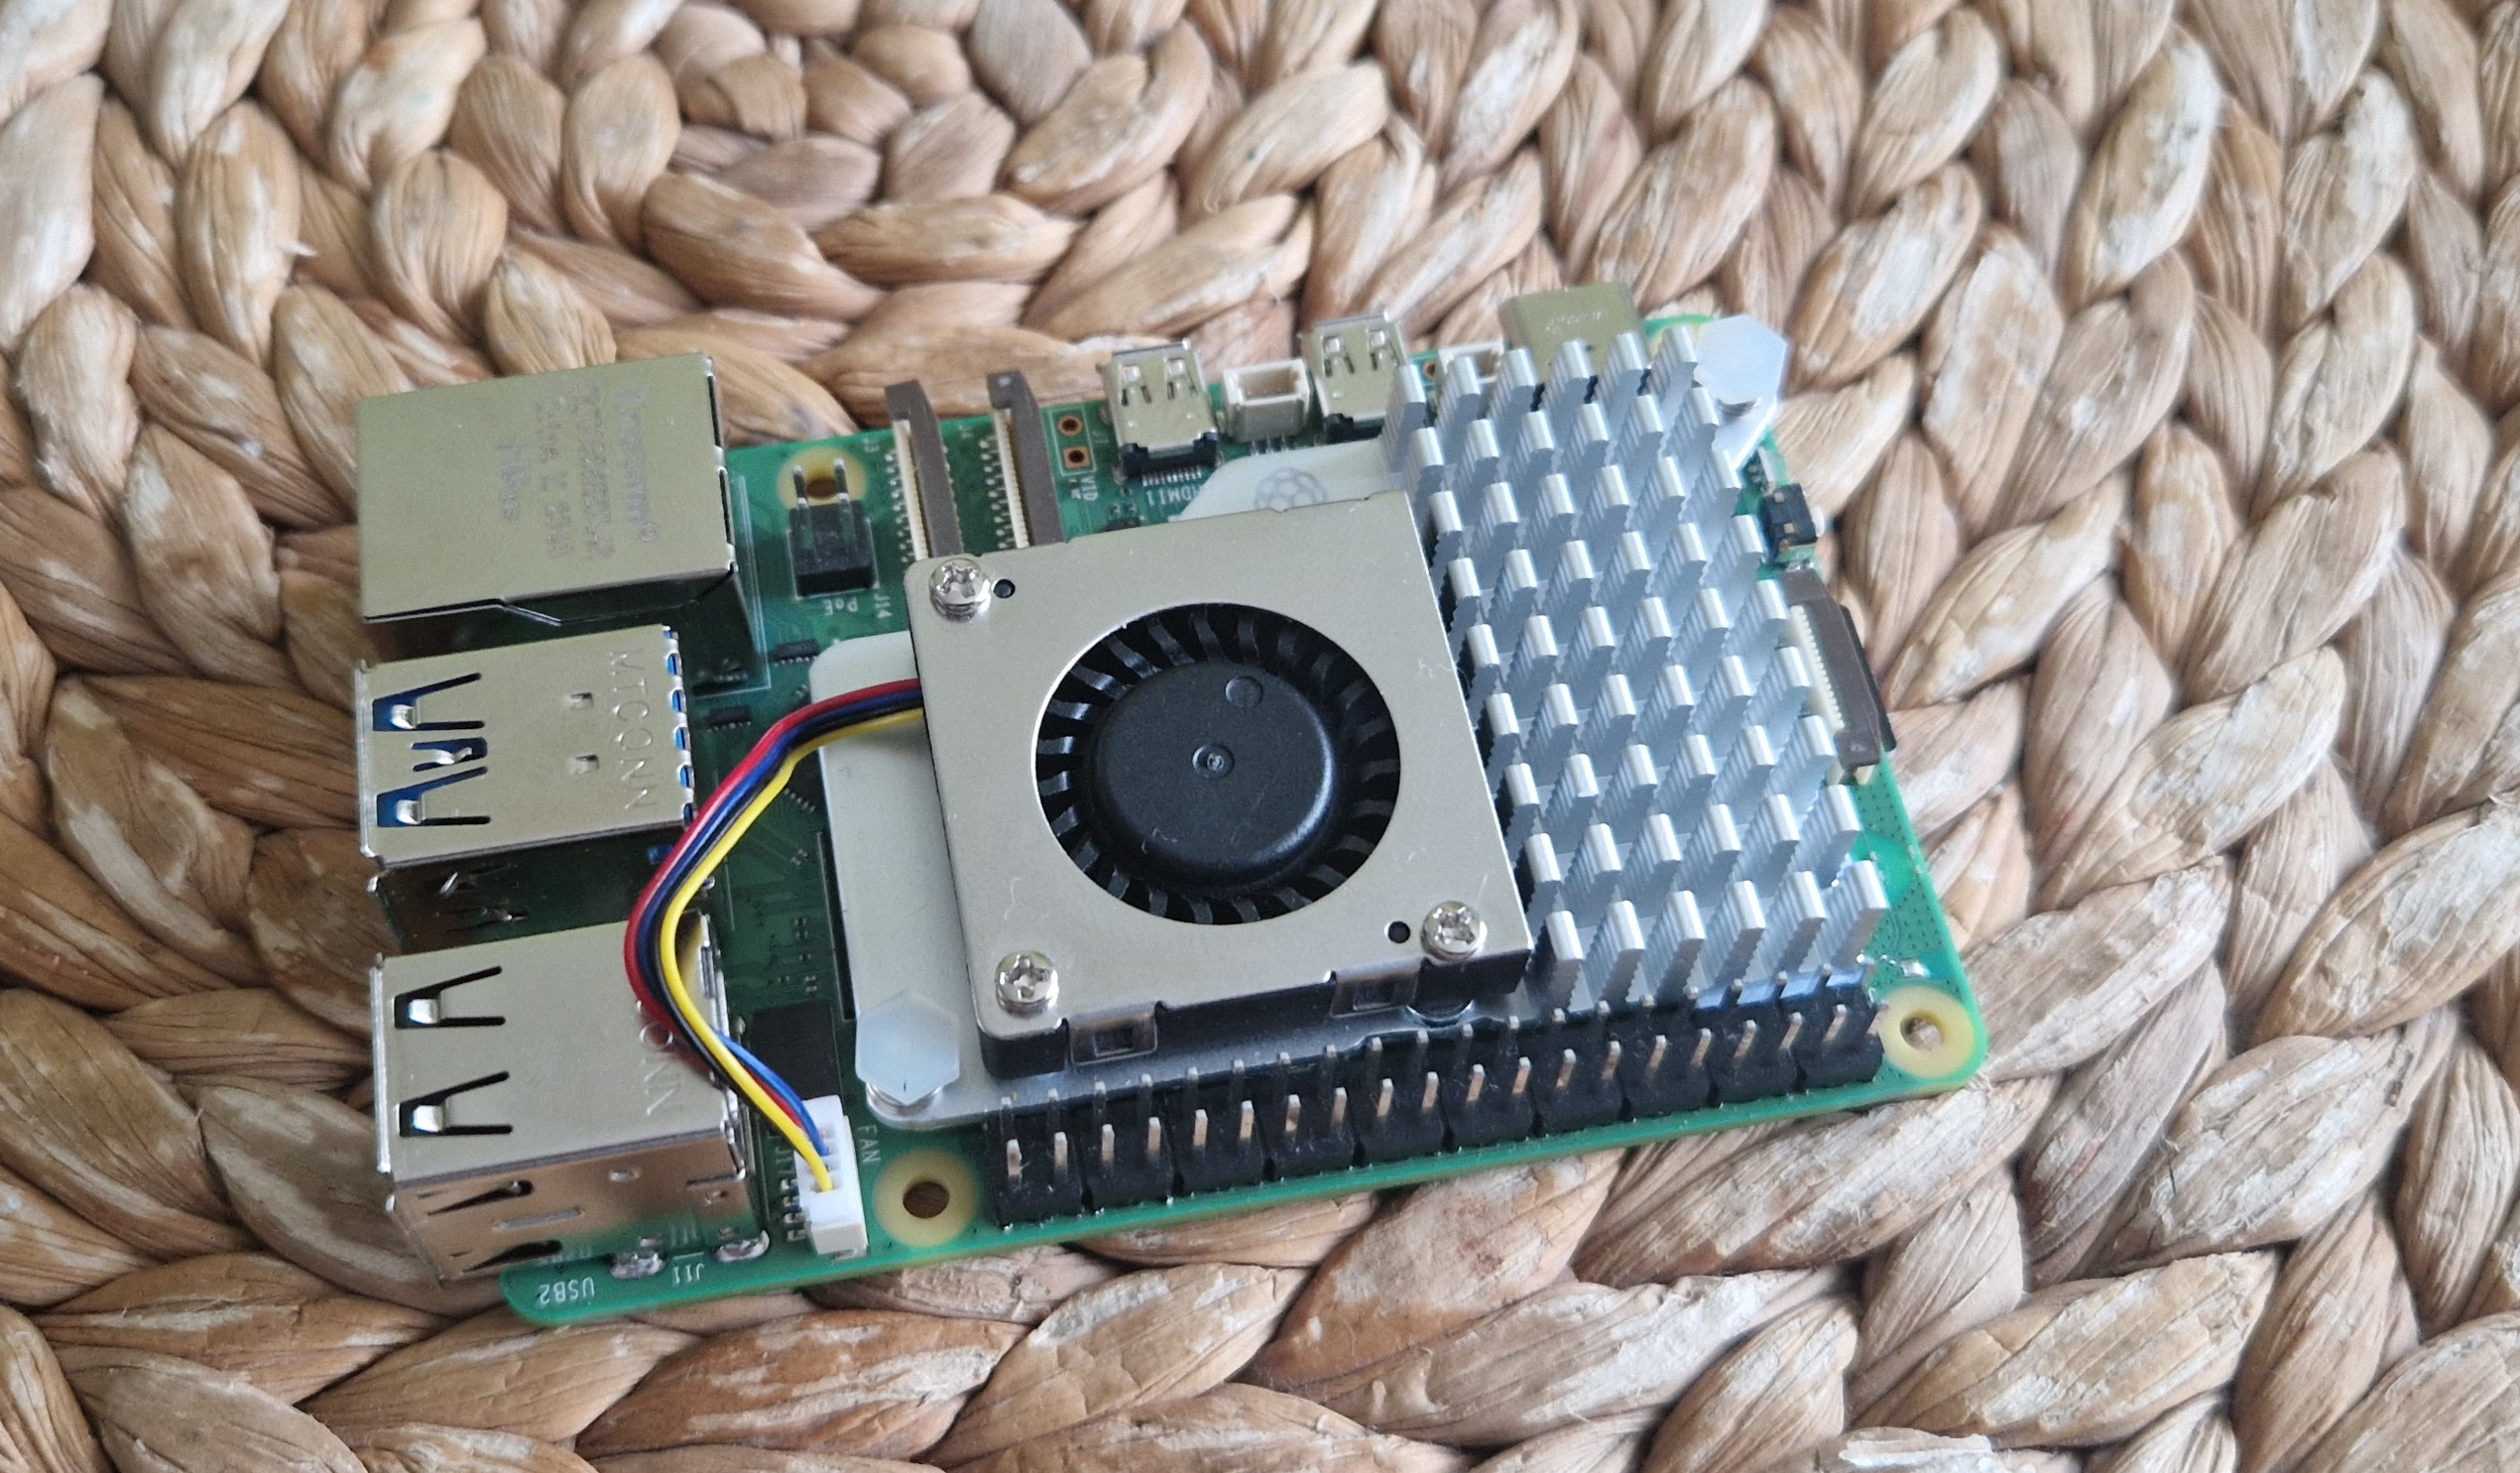
\includegraphics[width=0.4\textwidth]{img/rpi5-active-cooler-c.jpg}
	\caption{RPi 5 s aktivním chladičem}
\end{wrapfigure}
Jde o nejnovější verzi slavného mikropočítače, který má v sobě 4 jádrový ARM
procesor. Tuto desku jsem již vlastnil, byla pro mě tedy jasným favoritem.
Nakonec jsem ji použil právě pro tento projekt. Její spotřeba je opravdu nízká
a pohybuje se kolem 3 Wattů v nečinnosti.  \cite{RPi-Power}

\subsection{Server x86}

Rackové servery tradičního slova smyslu jsou pro projekty tohoto typu
více než vhodné. Zkušenosti se servery tohoto typu
jsem nasbíral na brigádách v lokálním ISP UnArtel. 

\subsection{NAS zařízení}

Komerční NAS zařízení, jako například od společností Synology a QNAP, nabízejí
uživatelsky přívětivé řešení pro síťové ukládání dat. Mezi jejich výhody patří
jednoduchost použití, snadné zapojení a konfigurace. Obvykle obsahují
integrovaný software pro zálohování, sdílení souborů a další funkce .  

Na druhou stranu, NAS zařízení mají i své nevýhody. Často používají proprietární
software, což omezuje možnosti přizpůsobení. Uživatel je také do jisté míry
vázán na ekosystém daného výrobce. Nižší modely mohou mít omezené možnosti
rozšíření. Navíc, použití komerčního NAS zařízení by pro tento projekt znamenalo
menší příležitost k praktickému učení se o konfiguraci hardwaru a softwaru ve
srovnání s vlastním sestavením systému . A co je nejdůležitější, pořizovací cena
komerčního NAS zařízení by byla pravděpodobně vyšší než náklady na komponenty
použité v tomto projektu, což by bylo v rozporu s cílem nízkonákladového řešení.  

\subsection{Závěr}



Na základě výše uvedených úvah jsem se rozhodl jako platformu pro svůj
zálohovací systém použít Raspberry Pi 5. Hlavním důvodem byla jeho dostupnost
, což přímo naplňuje
požadavek na nízké náklady. Dalším významným faktorem byla příležitost k získání
praktických zkušeností s konfigurací hardwaru a softwaru při stavbě vlastního
řešení.


\section{Jak připojit disk k RPI 5?}

Nevýhoda Raspberry Pi je absence SATA rozhraní pro připojení disků.
Musel jsem tak sáhnout po alternativním řešení v podobě 
USB-to-SATA adaptéru značky AXAGON. Tato česká značka nabízí 
velký sortiment příslušenství tohoto typu. Doma nám ležel v šuplíku
USB HDD Dock této značky, jehož využití pro mě 
bylo jasnou volbou.

Nejprve jsem ale musel vyzkoušet, jestli je tento dock kompatibilní 
s Raspberry Pi. Ukázalo se, že je připojení bezproblémové, a tak
jsem mohl začít testovat použité 2TB disky pocházející ze serverů
firmy UnArtel. Spouštěl jsem testy S.M.A.R.T. pomocí programu smartctl.

\begin{lstlisting}
smartctl -t short /dev/device
\end{lstlisting} 

Vypadalo to beznadějně, všechny disky vykazovaly vady. 
Naštěstí jsem ale našel jeden disk, který fungoval bezproblémově.
Připojil jsem ho k Raspberry Pi a pomocí nástroje
\emph{fdisk} jsem ho formátoval a vytvořil nové oddíly.
Poté jsem příkazem \emph{mkfs.ext4} udělal nový souborový systém.




\section{3D tištěný kryt}

Především kvůli ochraně před poškozením obvodů jsem se rozhodl 
sestrojit vlastní kryt. K návrhu jsem použil CAD software 
Autodesk Fusion 360, k němuž mám jako student přístup zdarma.
Hlavním cílem bylo spojit komponenty do jednoho celku.


\begin{figure}[h]
\centering
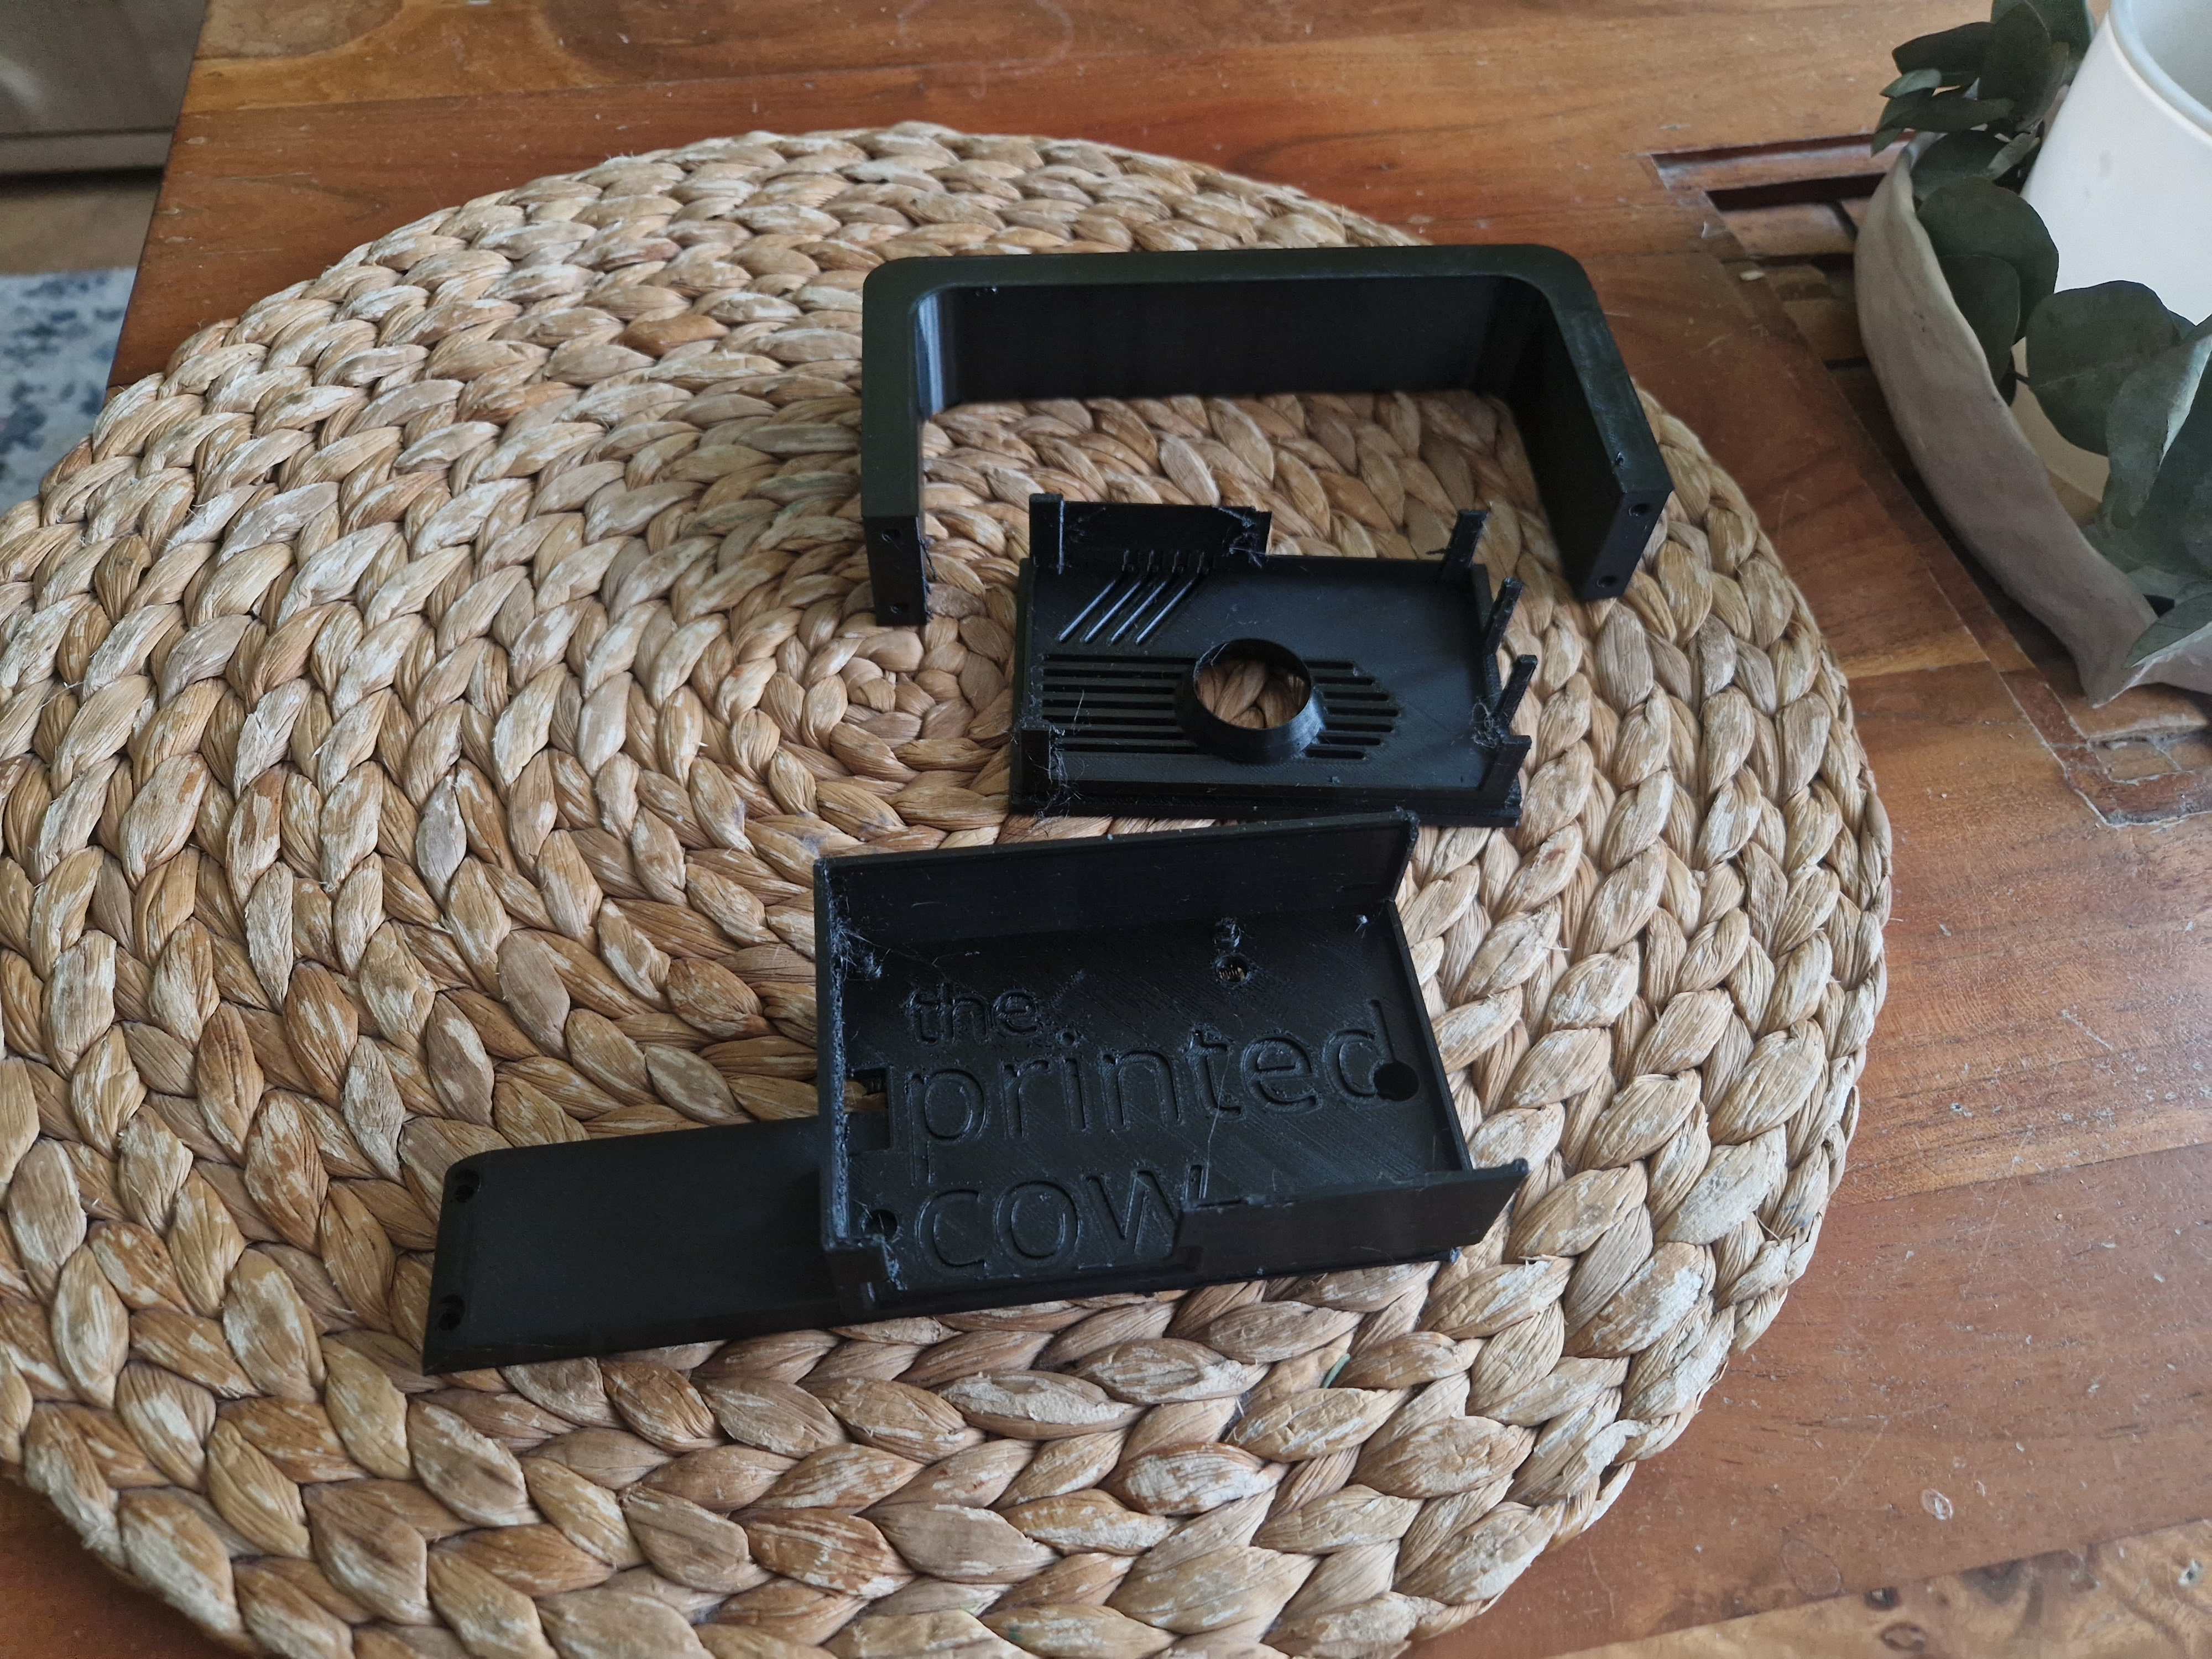
\includegraphics[width=0.8\textwidth]{img/dily-zvlast.jpg}
\caption{Díly vytišténé na 3D tiskárně}
\end{figure}

Důležitým prvkem návrhu je objímka, která pevně drží USB dokovací stanici.
Skládá se ze dvou dílů, které jsou spojeny šrouby M3. Jeden z dílů jsem
spojil s
\href{https://www.printables.com/model/705427-retro-raspberry-pi-5-case-snap-fit}{krytem
na Raspberry Pi}, který jsem našel na internetu.

\begin{figure}[h]
	\centering
	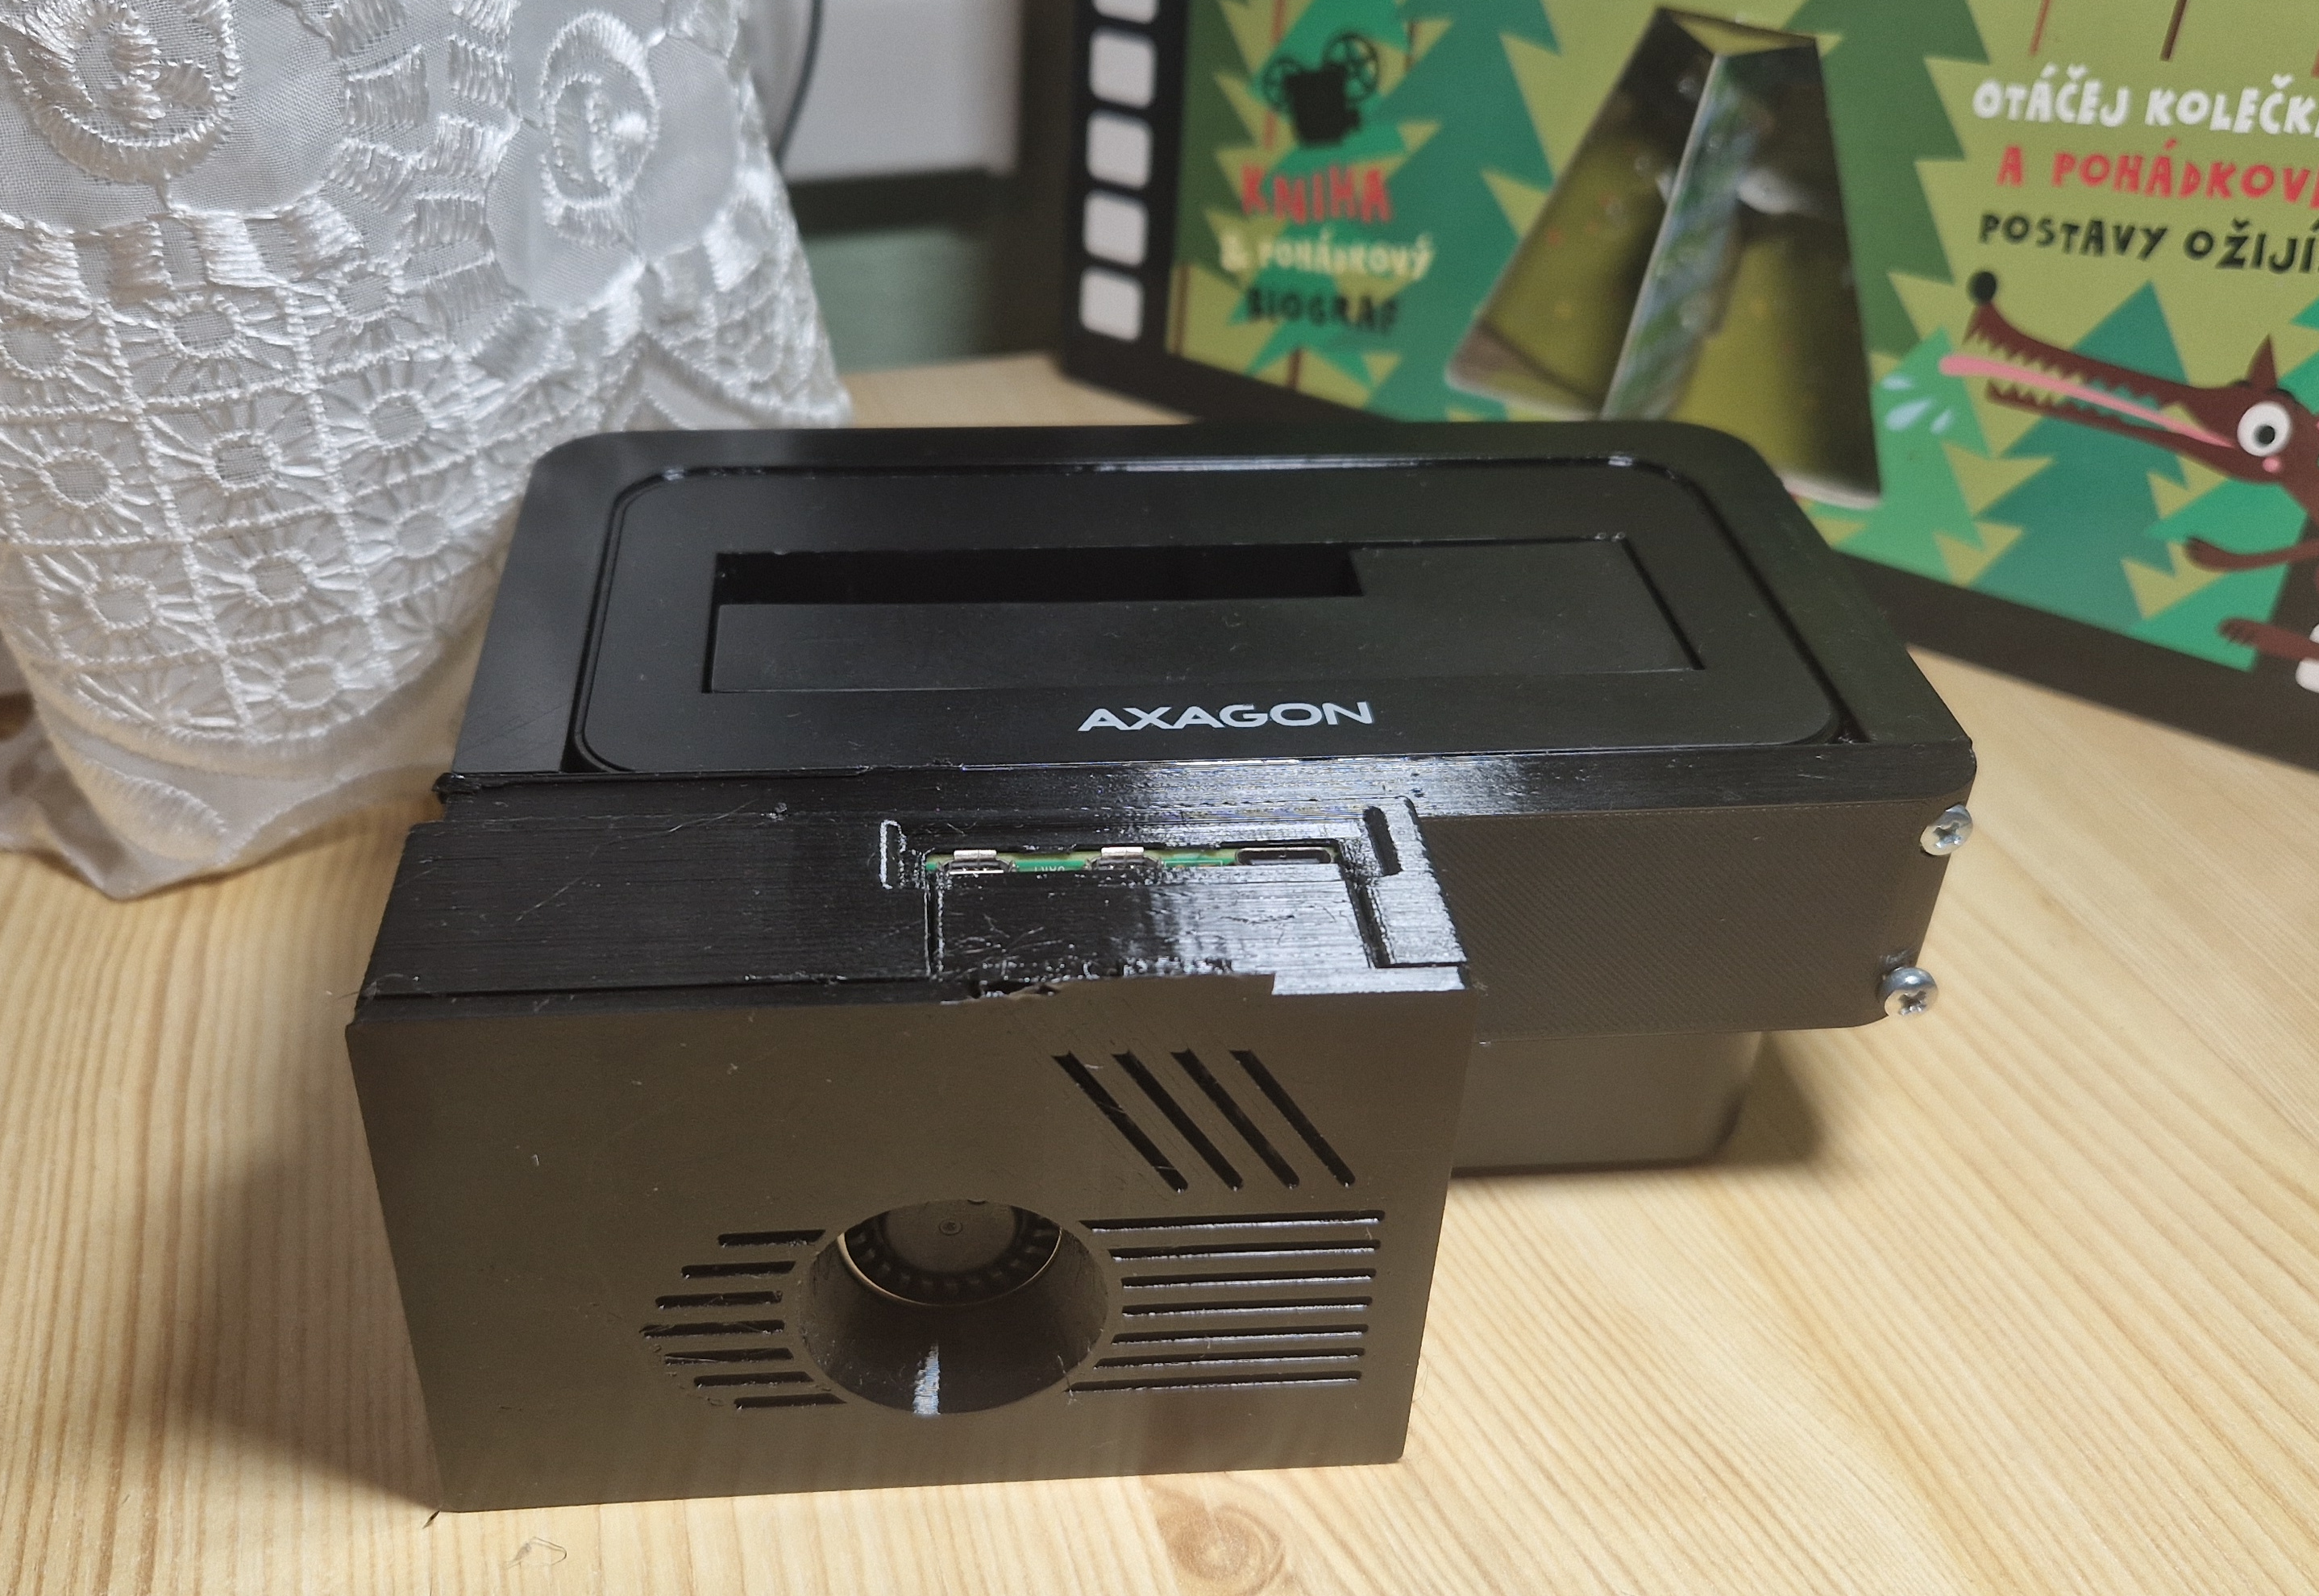
\includegraphics[width=1\textwidth]{img/skladani4-c.jpg}
	\caption{Sestavená zálohovací stanice}
	\end{figure}


Po sestavení těchto dílů vypadalo celé zařízení velmi esteticky. 
Podařilo se mi totiž napodobit tvar objímky i její barvu.
Problém nastal až v momentě, kdy jsem propojil jednotlivé komponenty. 
To přineslo kabelový chaos, který se mi zatím nepovedlo vyřešit.



\begin{figure}[h]
\centering
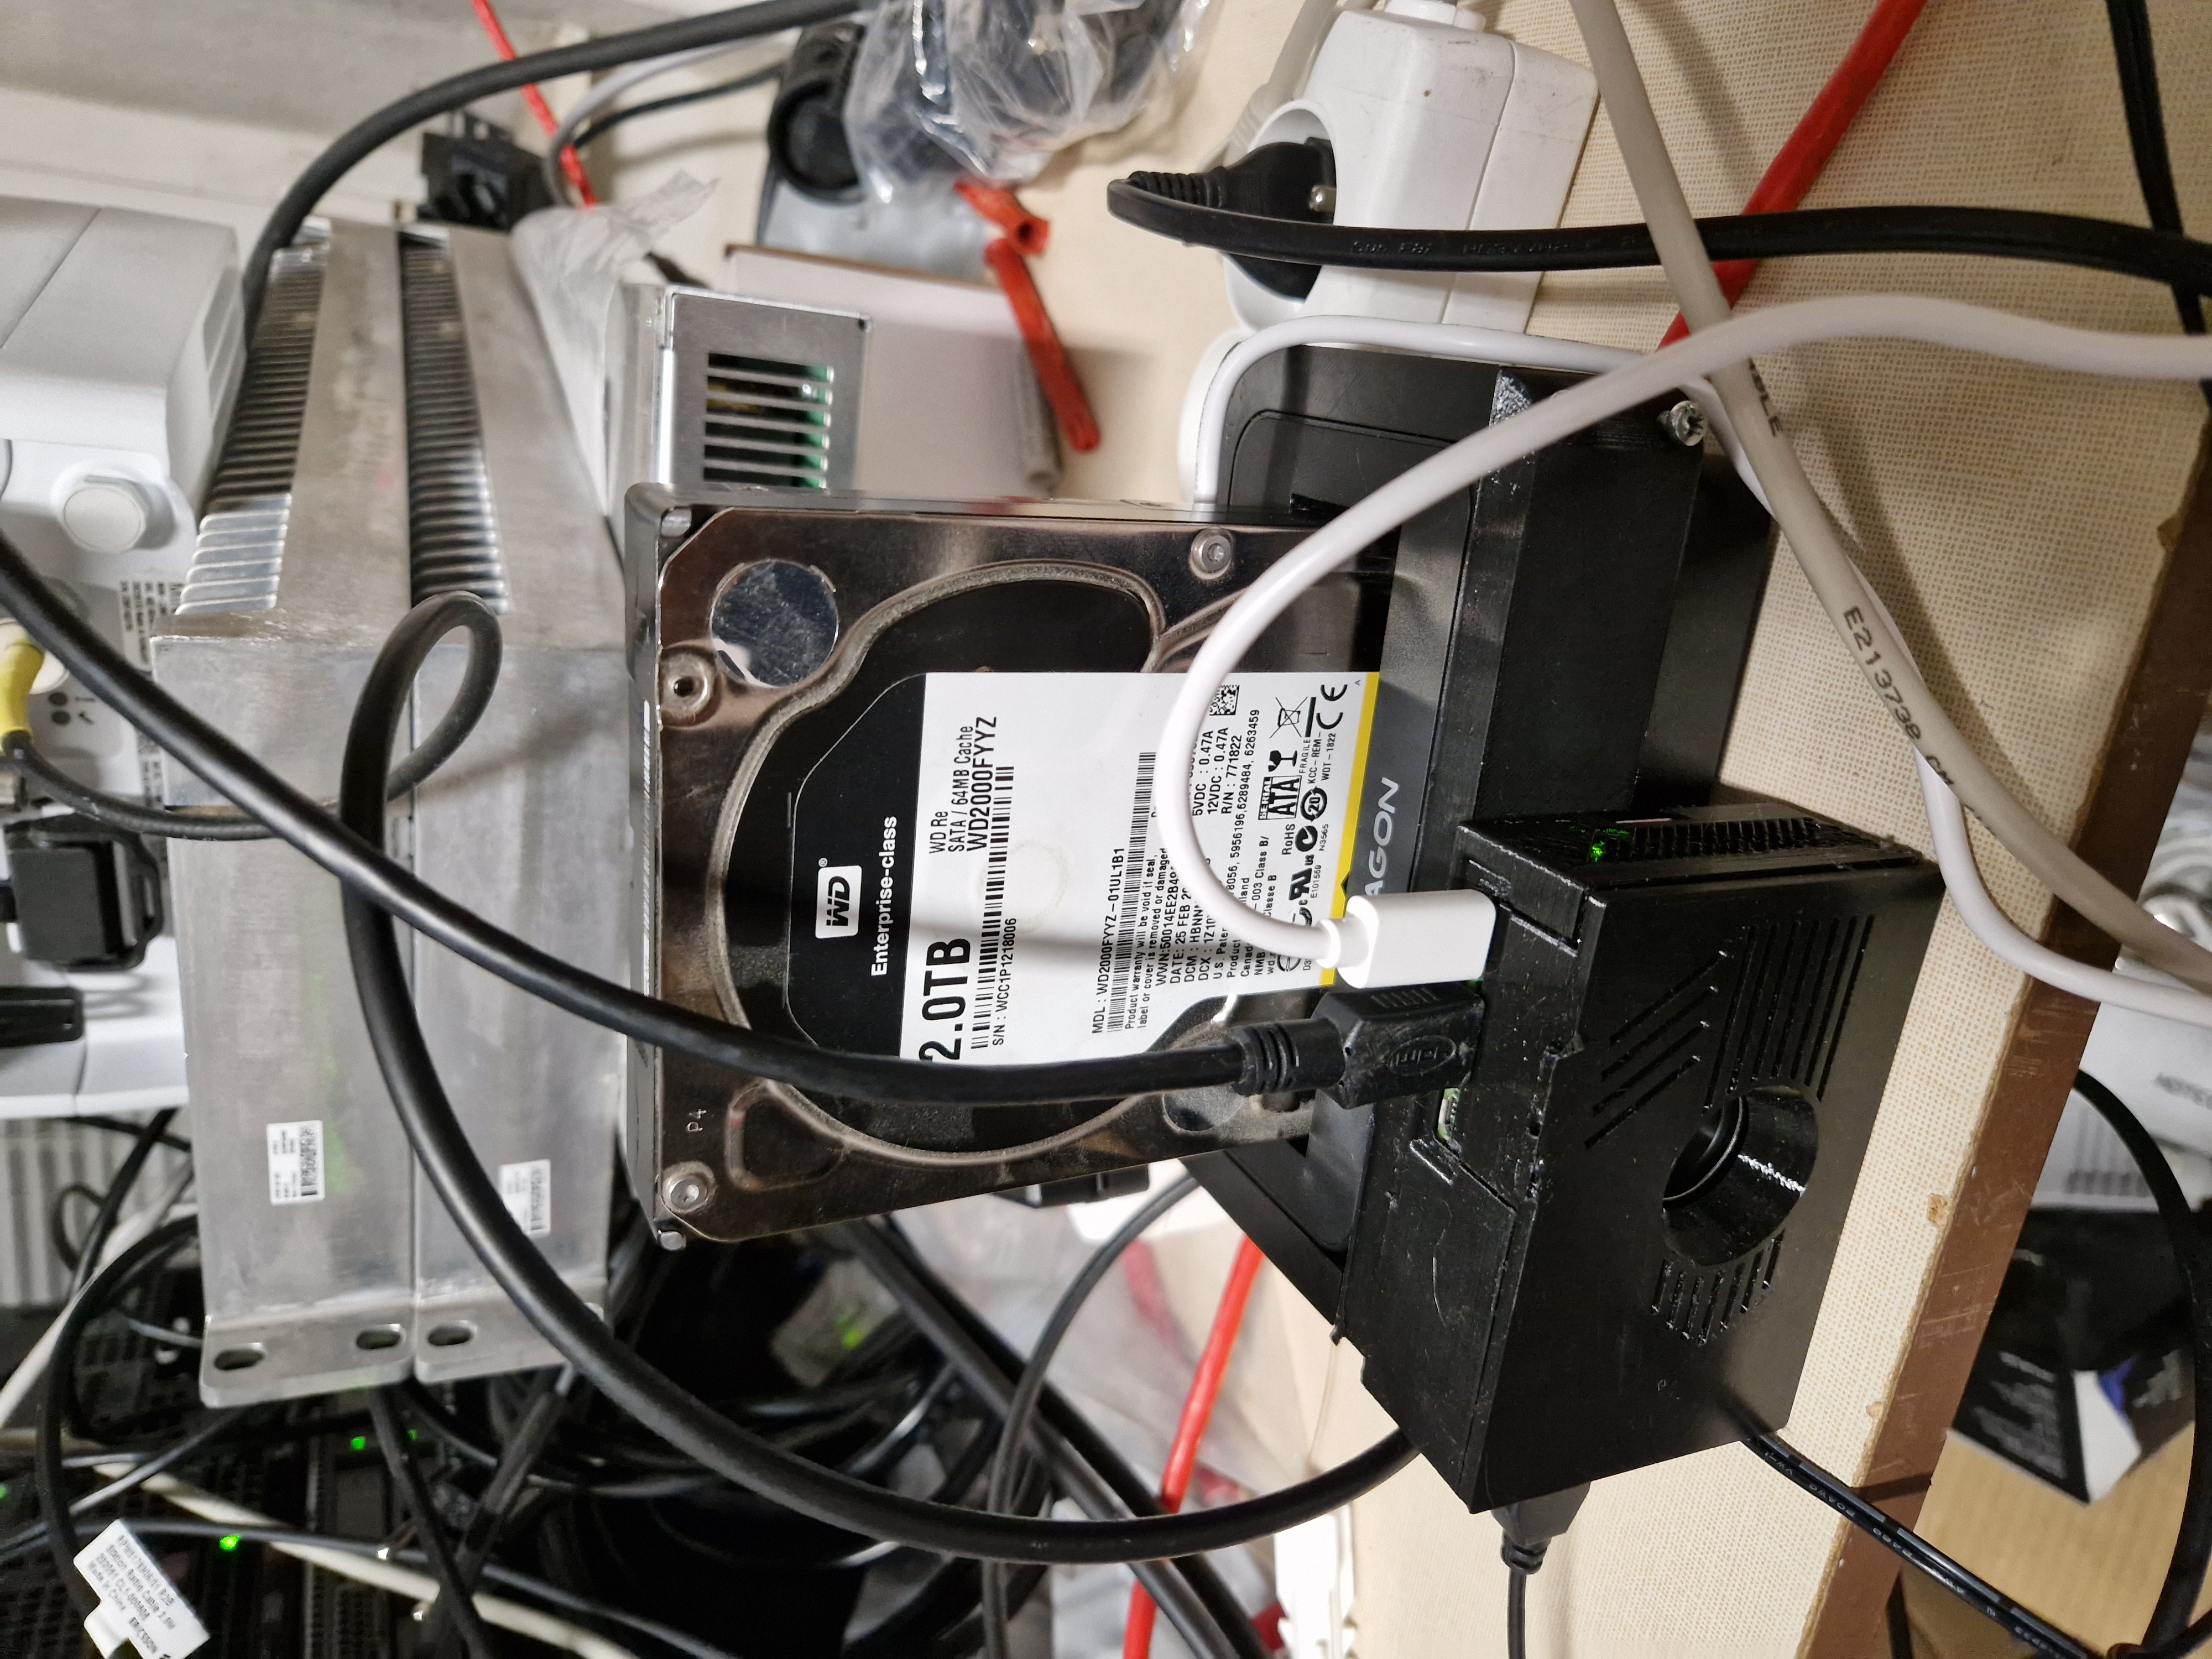
\includegraphics[width=0.9\textwidth]{img/zapojeni4.jpg}
\caption{Připojení všech komponent včetně disku}
\end{figure}


% TODO: kabely

% Umístnění UnArtel, Gigabit

\chapter{Software}

Pro správu zálohování bylo potřeba vybrat vhodný software. 
V úvahu přicházelo několik open-source řešení jako například 
Kopia, BorgBackup nebo Duplicati. Nakonec jsem vybral software 
Kopia. 

\begin{wrapfigure}{r}{0.4\textwidth}
	\centering
	
\includegraphics[width=0.4\textwidth]{img/kopia.jpg}
	\caption{Logo Kopia}
\end{wrapfigure}
Kopia je moderní nástroj, který vznikl v dílně Jarka Kowalského, 
programátora z Googlu. Používá jazyk Go a je velmi dobře optimalizovaný.
\cite{Kopia-GitHub}
Zálohy jsou vytvářeny ve formě inkrementálních snapshotů,
což znamená, že se po opakovaném spuštění nevytváří nová záloha, ale 
připíšou se pouze změny a nově přidané soubory. Podporuje deduplikaci,
díky čemuž je vícero kopií jednoho souboru ukládáno pouze jednou. 
Zálohy jsou automaticky komprimované a šifrované, takže se nejen ušetří 
místo, ale taky jsou data uložena bezpečně. \cite{Kopia-Docs} Zato však hlavním
tahákem pro mě byla podpora cloudu. Těší mě, když vím, že v případě vyčerpání
místa na 
zálohovacím HDD můžu v kopia změnit repozitář a začít tak zálohovat na 
Google Drive.
Kopia má celou řadu dalších výhod,
které jsou popsány v dokumentaci na \url{https://kopia.io/docs/}.





% SSH - vzdálené připojení k
% RPi, Public Key authentication

% Souborový systém
% SSHFS

% Psaní práce, Vim LaTex










\chapter{Závěr}





\nocite{*}
\printbibliography[
	heading=bibintoc,
	title={Seznam zdrojů}
]

\cleardoublepage
\listoffigures
% \phantomsection
\addcontentsline{toc}{chapter}{Seznam obrázků}




\end{document}

